\documentclass{article}
\usepackage[utf8]{inputenc}
\usepackage{enumitem}
\usepackage{amsmath}
\usepackage{amsfonts}
\usepackage{indentfirst}
\usepackage{tikz}

\title{Lista 2}
\author{SME0121 - Processos Estocásticos}
\date{2022}

\begin{document}

\maketitle

\section{Exercício}
Observação: há um erro na primeira linha da matriz. Assuma que $P_{00}=0.5$ para que a soma da primeira linha seja 1.
\begin{enumerate}[label=(\alph*)]

    \item Usando que $P(A\cap B)=P(A|B)P(B)$, as propriedades da cadeia de Markov e a matriz de probabilidade, temos que
    
    $$P(X_0=0\cap X_1=1\cap X_2=2) =$$
    $$P(X_2=2|X_1=1\cap X_0=0)P(X_1=1|X_0=0)P(X_0=0) =$$
    $$P(X_2=2|X_1=1)P(X_1=1|X_0=0)P(X_0=0) =$$
    $$P_{12}P_{01}P(X_0=0) = 0.4\times0.2 \times 0.3 = 0.024$$
    
    \item Semelhante ao item (a).
    
    $$P(X_2=1\cap X_3=1|X_1=0) =$$
    $$\frac{P(X_1=0\cap X_2=1\cap X_3=1)}{P(X_1=0)} =$$
    $$\frac{P(X_3=1|X_2=1)P(X_2=1|X_1=0)P(X_1=0)}{P(X_1=0)} =$$
    $$P_{11}P_{01} = 0.6\times 0.2 = 0.12$$
    
    \newpage
    
    \item Semelhante aos items (a) e (b).
    
    $$P(X_1=1\cap X_2=1|X_0=0) =$$
    $$\frac{P(X_0=0\cap X_1=1\cap X_2=1)}{P(X_0=0)} =$$
    $$\frac{P(X_2=1|X_1=1)P(X_1=1|X_0=0)P(X_0=0)}{P(X_0=0)} =$$
    $$P_{11}P_{01} = 0.6\times 0.2 = 0.12$$

    \item Semelhante aos itens anteriores.
    
    $$P(X_0=1\cap X_1=0\cap X_2=2|X_0=1) =$$
    $$\frac{P(X_0=1\cap X_1=0\cap X_2=2)}{P(X_0=1)} =$$
    $$\frac{P(X_2=2|X_1=0)P(X_1=0|X_0=1)P(X_0=1)}{P(X_0=1)} =$$
    $$P_{02}P_{10} = 0.3\times 0 = 0$$

\end{enumerate}

\section{Exercício}

\begin{enumerate}[label=(\alph*)]

    \item Temos que $P_{00}=\alpha$ e que $P_{10}=\beta$. Fora isso, sabemos que cada linha da matriz de transição soma 1 e que o espaço de estados possui apenas dois elementos, o que nos dá a seguinte matriz:
    $$\begin{bmatrix}
        \alpha & 1-\alpha\\
        \beta & 1-\beta
    \end{bmatrix}$$
    Para calcular a distribuição de equilíbrio, utilizamos as equações $\pi=\pi \mathbb{P}$ e $\sum_i{\pi_i}=1$.
    $$\begin{cases}
      \pi_0=\pi_0\alpha + \pi_1\beta\\
      \pi_0+\pi_1=1
    \end{cases}$$
    $$\begin{cases}
      \pi_0(1-\alpha)=\pi_1\beta\\
      \pi_1=1-\pi_0
    \end{cases}$$
    $$\pi_0(1-\alpha)=\beta-\beta\pi_0$$
    $$\pi_0=\frac{\beta}{\beta+1-\alpha}$$
    $$\pi_1=\frac{1-\alpha}{\beta+1-\alpha}$$
    
    \newpage
    
    \item O enunciado está mal formulado. Vamos assumir que queremos calcular $P(X_{n+4}=0|X_n=0)$.
    
    Assumindo que
    
    $$\mathbb{P}=\begin{bmatrix}
        0.7 & 0.3\\
        0.4 & 0.6
    \end{bmatrix}$$
    
    Temos que encontrar o termo $P_{00}$ de $\mathbb{P}^{4}$.
    
    $$\mathbb{P}^2=\begin{bmatrix}
        0.61 & 0.39\\
        0.52 & 0.48
    \end{bmatrix}$$
    
    $$\mathbb{P}^4=\begin{bmatrix}
        0.5749 & P_{01}\\
        P_{10} & P_{11}
    \end{bmatrix}$$
    
    Portanto, a probabilidade é de $57.49\%$.
    
    
    
\end{enumerate}

\section{Exercício}

\begin{enumerate}
    \item[] Temos que $Z_n=(X_{n-1},X_n)$. Logo, $Z_{n+1}=(X_n,X_{n+1})$. Isso significa que $Z_n$ e $Z_{n+1}$ compartilham de um estado $X_n$. Logo, temos que
    
    $$Q_{(a,b)(c,d)}=0,$$
    
    sempre que $b\neq c$.
    
    Definindo os estados $0\rightarrow (0,0)$, $1\rightarrow (0,1)$, $2\rightarrow (1,0)$ e $3\rightarrow (1,1)$, temos a seguinte matriz de probabilidades para $Z_n$:
    
    $$\mathbb{Q}=\begin{bmatrix}
        Q_{00} & Q_{01} & 0 & 0\\
        0 & 0 & Q_{12} & Q_{13}\\
        Q_{20} & Q_{21} & 0 & 0\\
        0 & 0 & Q_{32} & Q_{33}\\
    \end{bmatrix}$$
    
    Para $b=c$, temos que
    
    $$Q_{(a,b)(c,d)}=P(X_{n+1}=d\cap X_n=c|X_n=b\cap X_{n-1}=a) =$$
    $$P(X_{n+1}=d\cap X_n=c|X_n=b) =$$
    $$\frac{P(X_{n+1}=d\cap X_n=b)}{P(X_n=b)} =$$
    $$P(X_{n+1}=d|X_n=b) = P_{bd}.$$
    
    \newpage
    
    Dessa forma, temos por fim a matriz de probabilidade da variável aleatória $Z_n$:
    
    $$\mathbb{Q}=\begin{bmatrix}
        \alpha & 1-\alpha & 0 & 0\\
        0 & 0 & 1-\beta & \beta\\
        \alpha & 1-\alpha & 0 & 0\\
        0 & 0 & 1-\beta & \beta\\
    \end{bmatrix}$$
    
\end{enumerate}

\section{Exercício}

Observação: A frase ``a probabilidade do jogador A atingir estado i antes dele atingir o estado 0'' está incorreta nesse contexto. A frase correta deveria ser ``a probabilidade da fortuna do jogador A''.

Observação 2: Há um erro na lista em que o exercício atual possui duas questões (a). A segunda será encarada como (b).

Observação 3: Ficou ambígua a frase ``jogador A ganhe um dólar do jogador B antes que o jogador B ganhe 99 dólares do jogador A''. Isso foi questionado ao professor durante a aula e a interpretação correta segundo ele é: ``fortuna do jogador A antes da fortuna do jogador B''. Uma interpretação equivalente deve ser assumida para na questão (b).

\begin{enumerate}[label=(\alph*)]
    \item Resultado vem direto da equação fornecida.
    
    $$\alpha_{99} = \frac{(\frac{0.6}{0.4})^{99}-1}{(\frac{0.6}{0.4})^{100}-1} = \frac{2\cdot 3^{99}-2^{100}}{3\cdot 3^{99}-2^{100}}\approx \frac{2}{3}$$
    
    \item Novamente resultado vem direto da equação.
    
    $$1-\alpha_{98} = 1-\frac{(\frac{0.6}{0.4})^{98}-1}{(\frac{0.6}{0.4})^{100}-1} = \frac{5\cdot 3^{98}}{9\cdot 3^{98}-2^{100}}$$
    
    $$\frac{5\cdot 3^{98}}{9\cdot 3^{98}-2^{100}} > \frac{1}{2} \Leftrightarrow 3^{98} > -2^{100}$$
    
    Como a última inequação é claramente verdadeira, então a probabilidade da ruína de A nessa situação é maior que $50\%$. 

\end{enumerate}

\newpage

\section{Exercício}

\begin{enumerate}[label=(\alph*)]
    \item Para esta questão se usa as mesmas ferramentas que no exercício 1 desta mesma lista.
    
    $$P(X_0=0\cap X_1=0\cap X_2=0|X_0=0) =$$
    $$\frac{P(X_0=0\cap X_1=0\cap X_2=0)}{P(X_0=0)} =$$
    $$\frac{P(X_2=0|X_1=0)P(X_1=0|X_0=0)P(X_0=0)}{P(X_0=0)} =$$
    $${P_{00}}^2 = (1-\alpha)^2$$
    
    \item Aqui, deve-se considerar a matriz de probabilidade.
    
    $$\mathbb{P}=\begin{bmatrix}
        1-\alpha & \alpha\\
        \alpha & 1-\alpha
    \end{bmatrix}$$
    
    $$\mathbb{P}^2=\begin{bmatrix}
        2\alpha^2-2\alpha+1 & 2\alpha(1-\alpha)\\
        2\alpha(1-\alpha) & 2\alpha^2-2\alpha+1
    \end{bmatrix}$$
    
    A probabilidade $P(X_2=0|X_0=0)$ é igual a $2\alpha^2-2\alpha+1$.
    
    \item Para calcular a distribuição de equilíbrio, utilizamos as equações $\pi=\pi\mathbb{P}$ e $\sum_i{\pi_i}=1$, como feito anteriormente no exercício 2.
    
    $$\begin{cases}
      \pi_0=\pi_0(1-\alpha) + \pi_1\alpha\\
      \pi_0+\pi_1=1
    \end{cases}$$
    $$\begin{cases}
      \pi_0=\pi_0 - \pi_0\alpha + \pi_1\alpha\\
      \pi_1=1-\pi_0
    \end{cases}$$
    $$\pi_0=\pi_1=\frac{1}{2}$$
    
    \newpage
    
    \item Por fim, usa-se as multiplicações da matriz de probabilidade, de modo semelhante à questão (b) deste exercício.
    
    $$\mathbb{P}=\begin{bmatrix}
        0.9 & 0.1\\
        0.1 & 0.9
    \end{bmatrix}$$
    
    $$\mathbb{P}^2=\begin{bmatrix}
        0.82 & 0.18\\
        0.18 & 0.82
    \end{bmatrix}$$
    
    $$\mathbb{P}^4=\begin{bmatrix}
        0.7048 & 0.2952\\
        0.2952 & 0.7048
    \end{bmatrix}$$
    
    $$\mathbb{P}^5=\begin{bmatrix}
        P_{00} & P_{01}\\
        0.33616 & P_{11}
    \end{bmatrix}$$
    
    Ou seja, $P(X_5=0|X_0=1) = 33.62\%$

\end{enumerate}

\section{Exercício}

\begin{enumerate}[label=(\alph*)]
    \item Como cada linha da matriz soma 1,
    $$\begin{cases}
      x=0.3\\
      y=0.3\\
      z=0.4
    \end{cases}$$
    
    Gerando a matriz
    
    $$\mathbb{P}=\begin{bmatrix}
        0.6 & 0.3 & 0.1\\
        0.3 & 0.4 & 0.3\\
        0.4 & 0.1 & 0.5\\
    \end{bmatrix}$$
    
    A distribuição de equilíbrio é calculada por $\pi=\pi\mathbb{P}$ e $\sum_i{\pi_i}=1$.
    
    $$\begin{cases}
      \pi_0 = 0.6\pi_0+0.3\pi_1+0.4\pi_2\\
      \pi_1 = 0.3\pi_0+0.4\pi_1+0.1\pi_2\\
      1 = \pi_0 + \pi_1 + \pi_2
    \end{cases}$$
    
    Usando qualquer método de resolução de sistemas, se obtém o seguinte resultado:
    
    $$\pi=(\frac{27}{58}, \frac{16}{58}, \frac{15}{58})$$

    \newpage

    \item Usando as técnicas do exercício 1 desta lista, temos
    
    $$P(X_0=0\cap X_1=1\cap X_2=2) = $$
    $$P(X_2=2|X_1=1)P(X_1=1|X_0=0)P(X_0=0) = $$
    $$P_{12}P_{01}p_0 = 0.3\cdot 0.3\cdot 0.3 = 0.027$$
    
    e

    $$P(X_2=1\cap X_3=1|X_1=0) = $$
    $$\frac{P(X_1=0\cap X_2=1\cap X_3=1)}{P(X_1=0)} = $$
    $$\frac{P(X_3=1|X_2=1)P(X_2=1|X_1=0)P(X_1=0)}{P(X_1=0)} = $$
    $$P_{11}P_{01} = 0.4\cdot 0.3 = 0.12$$
    
    \item O enunciado nos manda determinar $P(X_0=1\cap X_1=0\cap X_2=2|X_0=1)$. Podemos proceder exatamente como na questão (d) do exercício 1 desta lista.
    
    $$P(X_0=1\cap X_1=0\cap X_2=2|X_0=1) =$$
    $$\frac{P(X_0=1\cap X_1=0\cap X_2=2)}{P(X_0=1)} =$$
    $$P_{02}P_{10} = 0.1\cdot 0.3 = 0.03$$

\end{enumerate}

\section{Exercício}

\begin{enumerate}[label=(\alph*)]
    \item Novamente, calcular a distribuição de equilíbrio.
    
    $$\begin{cases}
      \pi_0 = 0.8\pi_0+0.1\pi_1\\
      \pi_1 = 0.1\pi_0+0.7\pi_1+0.1\pi_2\\
      1 = \pi_0 + \pi_1 + \pi_2
    \end{cases}$$
    
    $$\begin{cases}
      \pi_0 = 0.125\\
      \pi_1 = 0.25\\
      \pi_2 = 0.625
    \end{cases}$$
    
    \newpage
    
    \item O que o enunciado pede para calcular é $\mathbb{P}^2$.
    
    $$\mathbb{P}^2=\begin{bmatrix}
        0.65 & 0.16 & 0.19\\
        0.15 & 0.52 & 0.33\\
        0.01 & 0.16 & 0.83
    \end{bmatrix}$$

\end{enumerate}

\section{Exercício}

\begin{enumerate}[label=(\alph*)]
    \item Como nenhum dos estados se comunicam, há 3 classes: $\{0\}$, $\{1\}$ e $\{2\}$.
    \item Não, cadeias irredutíveis por definição possuem apenas 1 classe.
    \item Uma das condições para se encontrar a distribuição de equilíbrio de uma cadeia é a sua irredutibilidade. Não é o caso, pois a cadeia não é irredutível.

\end{enumerate}

\section{Exercício}

\begin{enumerate}
    \item[] A cadeia possui 2 estados: $\{0,1\}$ e $\{2\}$, pois o estado 2 não se comunica com nenhum dos outros estados. Dessa forma, a cadeia não é irredutível, e não satisfaz uma das condições para encontrar a distribuição de equilíbrio.

\end{enumerate}

\section{Exercício}

Observação: Esse exercício não deixa claro no enunciado se, em um fim de semana, se conta o número de câmeras para determinar o estado e depois se realiza a política, ou se primeiro se realiza a política e depois se determina o estado. Vamos considerar que primeiro se determina o estado e depois se realiza a política, pois caso contrário, o estado 0 seria inatingível.

Observação 2: Provavelmente a linha 1 e 2 estão trocadas. Vamos considerar a seguinte matriz de probabilidades:

$$\mathbb{P}=\begin{bmatrix}
    0.080 & 0.184 & 0.368 & 0.368\\
    0.632 & 0.368 & 0 & 0\\
    0.264 & 0.368 & 0.368 & 0\\
    0.080 & 0.184 & 0.368 & 0.368
\end{bmatrix}$$

Isso porque, dado o enunciado e nossa interpretação comentada na observação anterior, faz sentido que não haja chance da cadeia ir do estado 1 para o estado 2 em um passo. 

\newpage

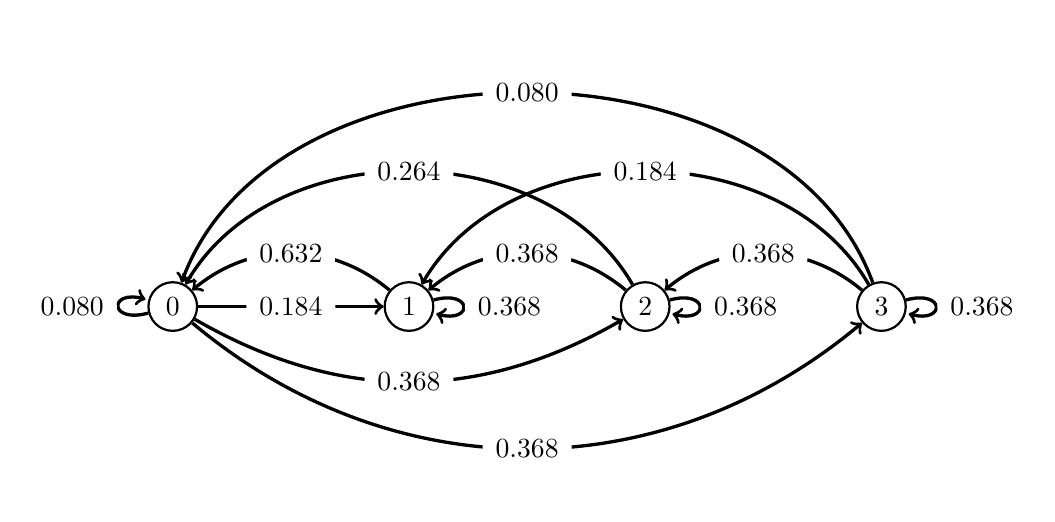
\begin{tikzpicture}
    \begin{scope}[every node/.style={circle,thick,draw}]
        \node (0) at (0,0) {0};
        \node (1) at (3,0) {1};
        \node (2) at (6,0) {2};
        \node (3) at (9,0) {3};
    \end{scope}
    
    \begin{scope}[every node/.style={fill=white,circle},
                  every edge/.style={draw=black,very thick}]
        \path [->] (0) edge node {$0.184$} (1);
        \path [->] (0) edge[bend right=30] node {$0.368$} (2);
        \path [->] (0) edge[bend right=40] node {$0.368$} (3);
        
        \path [->] (1) edge[bend right=40] node {$0.632$} (0);
        \path [->] (2) edge[bend right=40] node {$0.368$} (1);
        \path [->] (2) edge[bend right=60] node {$0.264$} (0);
        \path [->] (3) edge[bend right=70] node {$0.080$} (0);
        \path [->] (3) edge[bend right=60] node {$0.184$} (1);
        \path [->] (3) edge[bend right=40] node {$0.368$} (2);
        
        \draw [->] (0) edge[loop left] node {$0.080$} (0);
        \draw [->] (1) edge[loop right] node {$0.368$} (1);
        \draw [->] (2) edge[loop right] node {$0.368$} (2);
        \draw [->] (3) edge[loop right] node {$0.368$} (3);
    \end{scope}
\end{tikzpicture}

\begin{enumerate}[label=(\alph*)]
    
    \item Grafo desenhado acima.

    \item Sim, pois todo estado se comunica com outro estado, o que faz com que a cadeia tenha apenas uma classe, e portanto seja irredutível.
    
    \item Cálculo da distribuição de equilíbrio.
    
    $$\begin{cases}
      \pi_1 = 0.184\pi_0+0.368\pi_1+0.368\pi_2+0.184\pi_3\\
      \pi_2 = 0.368\pi_0+0.368\pi_2+0.368\pi_3\\
      \pi_3 = 0.368\pi_0+0.368\pi_3\\
      1 = \pi_0+\pi_1+\pi_2+\pi_3
    \end{cases}$$
    $$\begin{cases}
      \pi_0 \approx 0.2857\\
      \pi_1 \approx 0.2849\\
      \pi_2 \approx 0.2632\\
      \pi_3 \approx 0.1664
    \end{cases}$$
    
    
    \item O tempo de recorrência é calculado por $\mu_i=\frac{1}{\pi_i}$. Temos então que $\mu_3 \approx 6.01$ semanas.

\end{enumerate}

\end{document}